\documentclass{standalone}
\usepackage{tikz}

\begin{document}

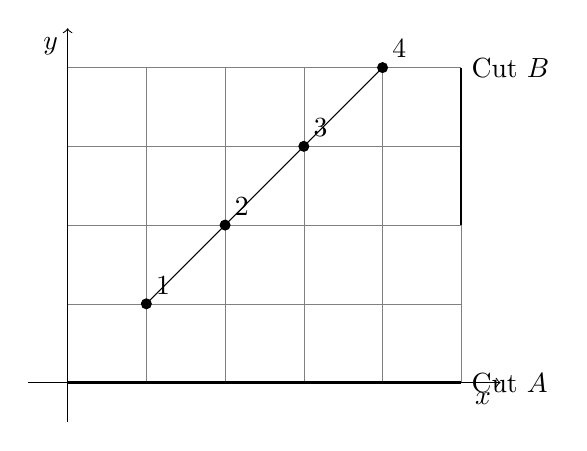
\begin{tikzpicture}[scale=1]
    % Grid
    \draw[help lines] (0,0) grid (5,4);
    
    % Points
    \fill (1,1) circle (2pt) node[anchor=south west] {1};
    \fill (2,2) circle (2pt) node[anchor=south west] {2};
    \fill (3,3) circle (2pt) node[anchor=south west] {3};
    \fill (4,4) circle (2pt) node[anchor=south west] {4};
    
    % Lines
    \draw (1,1) -- (2,2) -- (3,3) -- (4,4);
    
    % Labels for cuts
    \draw[thick] (5,2) -- (5,4) node[right] {Cut $B$};
    \draw[thick] (0,0) -- (5,0) node[right] {Cut $A$};
    
    % Axes
    \draw[->] (-0.5,0) -- (5.5,0) node[below left] {$x$};
    \draw[->] (0,-0.5) -- (0,4.5) node[below left] {$y$};
    
\end{tikzpicture}

\end{document}